%=======================================================================================%
% the main points of this introduction are 
% outline the complexity of biological systems for physicists
% 	> even though our theoretical models should preidct everything on the energy and length scales of biology we can't because of their heterogeneity.
%   > Give examples of the heterogenaity 
% Give some points on the history of molecular biophysics  
%   >  Hodgkin-Huxley Models
%   > Gramicidin 
% Point out how Cystic Fibrosis is an expression of this progression, going from genotype to phenotype using an ion channel to teach us biophysics. 
% conclusion.
\pagenumbering{arabic}
\chapter*{Foreword}
\setcounter{page}{1}
\label{chap:foreward}
\chapquote{} {}
\vspace

The more I wrote this thesis the more I found myself writing for my past self, so I think this thesis will be best read by my future students. If you've a loose grasp of second year undergaduate physics you should feel fairly at home reading this thesis. What will be less familiar to you the breadth of pre requisits to understand teh contents. What I have not had time to do is write an introduction to molecular biology, so there may be much chemistry missed by my students. So I reccomend a physics based introduction to those concepts such as those found in \cite{phillips2012}. On this note of pedagogy, care is taken to name certain authors to give the reader a kind of anchor for where to look in the literature.  

The past few years I have been captivated by the unending complexity in biological systems. If you need some inspiration please take this opportunity treat yourself to the fabulous work of \href {https://pdb101.rcsb.org/sci-art/goodsell-gallery}{David Goodsel} \cite{goodsell2009, goodsell2018, goodsell2020}. I've found that the mindset for solving biological problems feels very different to the focus we cultivate in students when they study idealised problems in mathematics and physics. The problems are broader. For example, plasma physicists may use the same mathematical tools to describe materials as diverse as the dense stellar core to the sparse intergalactic nebulae. These objects span 28 orders of magnitude in density \cite{chen2018}. Would that we were so lucky in biology, where we struggle to apply same physical models to deal with phenomena across a single order of magnitude. This diversity means we need many hands to solve problems in biology. Note that all the publications arising from this thesis have many many authors. Each researcher specialises not unlike, cells in a complex organism, in a specific discipline, but we all work together to produce the research.

If the reader is anything like myself they will find the amount assumed knowledge in biology daunting. It is quite difficult at first to figure out what questions to even ask or even figure out which subfield is causing us confusion. These difficulties are best alleviated by cultivating a broad coalition of connections, speak to medical doctors, clinicians, molecular biologists, biochemists \footnote{These last two are in fact different subfields but like many in this list it'll take you some time to understand the subtle differences which define each one.}, cell biologists, geneticists, bioinformaticians, theoretical chemists, computer scientists, neuroscientists, physicists, mathematicians, everyone. It will take time but remain patient and you will eventually find that a physics motivated approach can indeed explain and often even predict outcomes in biological experiments. A broad world view awaits you and it's really quite fun. 

A physics focussed review of the literature in the introductory chapter \ref{chap:introduction} and chapter \ref{chap:methods} will hopefully serve as a road map for my future students. The issue is that the field is now progressing so quickly that I'm sure much of this thesis will be out of date by the time I've given it to a student to read. 

The heterogeneity of biology is easy to observe. If you look at your arm, you will notice hair, pores, dry skin, dead skin, perhaps even tendons and muscles twitching beneath the surface. If you were to take a single cell from just beneath the skin and stain it to distinguish features in an electron microscope, you would find all sorts of complex structures called organelles. The size, shape and function of these elements would be different if the cell was taken from somewhere else in your body. Within and between each those organelles is a salty, wet dance of molecules large and small. This journey from your arm to your organelles spans 5 orders of magnitude. The complexity across length scales hints at the reasons behind biology's physical complexity. 


\begin{figure}
	\begin{center}
		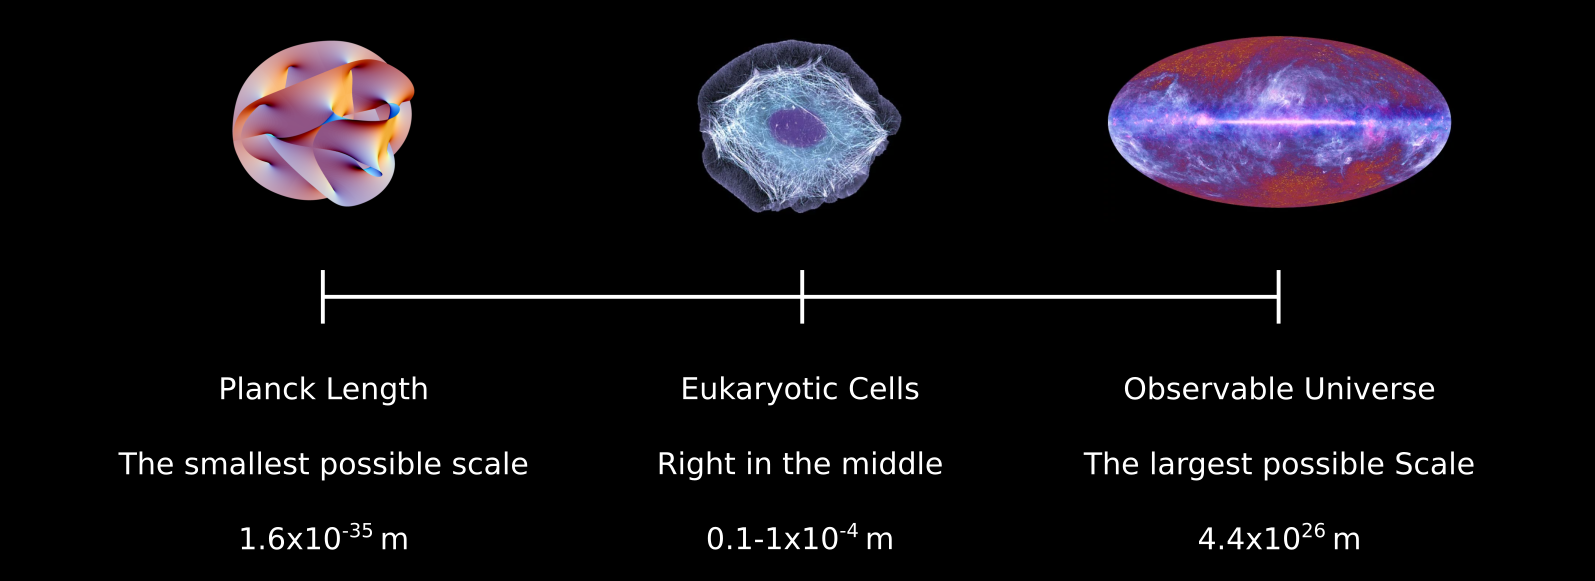
\includegraphics[width=1.0\textwidth]{figures/scales.png}
	\end{center}
	\captionsetup{singlelinecheck = false, justification=raggedright}
	\caption[The strange position that biological phenomenon occupy compared to the rest of physics] {\textbf{The strange position that biological phenomenon occupy compared to the rest of physics}}{It just so happens that if you plot the size of everything  in the universe on a log scale, eukaryotic cells fall right in the middle. A physicist can talk about both ends of this scale, we should learn something about the middle too.}
	\label{biology_scales}
\end{figure}

This thesis represents an all consuming effort by a single PhD student to make incremental on a single protein. There are 23000 different proteins in the human body and glimpsing the unprecedented complexity in a single one has been on the most existential experiences of my life. There is so much to do. In any case, good luck, bring a towel \cite{adams1979}. 
